\documentclass[10pt]{article}
\usepackage[margin=1in, paperwidth=8.5in, paperheight=11in]{geometry}
\usepackage{ifpdf,amsmath, amssymb, comment, color, graphicx, stmaryrd,setspace,enumitem,tikz, fancyhdr, wrapfig, textcomp, units, mathptmx, pdfpages, cancel, multicol}
\usepackage{hyperref}
\hypersetup{
    colorlinks=true,
    urlcolor=blue,
}

\setlength{\headheight}{14.5pt}
\newcommand{\Q}{\mathbb{Q}}
\newcommand{\R}{\mathbb{R}}
\newcommand{\Z}{\mathbb{Z}}
\newcommand{\vu}{\mathbf{u}}
\newcommand{\vv}{\mathbf{v}}
\newcommand{\vw}{\mathbf{w}}
\newcommand{\vi}{\mathbf{i}}
\newcommand{\vj}{\mathbf{j}}
\newcommand{\vk}{\mathbf{k}}
\newcommand{\vn}{\mathbf{n}}
\newcommand{\vr}{\mathbf{r}}
\newcommand{\va}{\mathbf{a}}
\newcommand{\vF}{\mathbf{F}}
\newcommand{\vL}{\mathbf{L}}
\newcommand{\vT}{\mathbf{T}}
\newcommand{\vN}{\mathbf{N}}
\newcommand{\proj}{\operatorname{proj}}
\newcommand{\orth}{\operatorname{orth}}
\newcommand\del\nabla
\newcommand\dotp[1][.5]{\,\mathbin{\vcenter{\hbox{\scalebox{#1}{$\bullet$}}}}\,}
\newcommand{\slice}{_\text{slice}}

% Solution text is in red. If you want the solutions to show, remove the \iffalse from the definition of the \red command.
%\newcommand{\red}[1]{ %\iffalse
%	\textcolor{red}{#1} }%\fi}

\newenvironment{red}{\color{red}}{\ignorespacesafterend}
\newenvironment{blue}{\color{blue}}{\ignorespacesafterend}
\newcommand{\green}[1]{\textcolor{green}{#1}}
\renewcommand{\section}[1]{\begin{center} \textbf{#1} \\\end{center}}
%
\hyphenpenalty=5000
\setlength{\parindent}{0in}
%\oddsidemargin=-.25in
\allowdisplaybreaks
\pagestyle{fancy}
\renewcommand{\headrulewidth}{0pt}
\lhead{MATH 202}
\rhead{Spring 2024}
%\lfoot{\copyright\ CLEAR Calculus 2010}
\cfoot{}

\begin{document}
%


%\onehalfspacing
\allowdisplaybreaks
%##################################################################
\section{PS\#10: Solutions to differential equations (part 2!) - \red{Answer key} }


Consider the differential equation $\displaystyle \frac{dy}{dt} = y-t$.

\begin{enumerate}[leftmargin=0pt]

\item (Modified from \href{https://activecalculus.org/single/sec-7-1-diff-eq-intro.html#mvy}{AC 7.1 Exercise 6}) A magic seashell has whispered into our ear that the following functions might be solutions to the differential equation. However, it is a \textit{rude} magic seashell which sometimes lies. Determine whether each of the following functions is a solution to the differential equation:


\begin{enumerate}
    \item $y(t) = t-2e^t+1$
    
    \begin{red}
    The LHS of the differential equation is $\dfrac{dy}{dt}$, which in this case is $1-2e^t+0$. 
    
    The RHS of the differential equation is $y-t$, which in this case is $\left(t-2e^t+1\right)-t = 1-2e^t$. 
    
    So, this \textbf{is a solution}, yay, because the LHS and the RHS match.
    \end{red}
    \item $y(t) = t+1$
    
    \begin{red}
    The LHS of the differential equation is $\dfrac{dy}{dt}$, which in this case is $1 + 0$. 
    
    The RHS of the differential equation is $y-t$, which in this case is $\left(t+1\right)-t = 1$. 
    
    So, this \textbf{is a solution}, yay, because the LHS and the RHS match.
    \end{red}

    \item $y(t) = 2e^t$

    \begin{red}
    The LHS of the differential equation is $\dfrac{dy}{dt}$, which in this case is $2e^t$. 
    
    The RHS of the differential equation is $y-t$, which in this case is $\left(2e^t\right)-t$. 
    
    So, this \textbf{is not a solution}, boo, because the LHS and the RHS \textbf{don't} match.
    \end{red}
    \item $y(t) = 1+\frac{e^t}{2}+t$
    
    \begin{red}
    The LHS of the differential equation is $\dfrac{dy}{dt}$, which in this case is $0 + \frac{e^t}{2}+1$. 
    
    The RHS of the differential equation is $y-t$, which in this case is $\left(1+\frac{e^t}{2}+t\right)-t = 1+\frac{e^t}{2}$. 
    
    So, this \textbf{is a solution}, yay, because the LHS and the RHS match.
    \end{red}
\end{enumerate}

\item One of the correct solutions in \#1 is the exact solution to the initial value problem $\dfrac{dy}{dt} = y-t$, $y(0) = -1$. Which one, and how can you tell?

\begin{red}
$y(t) = t + 1 - 2e^t$. I can tell because, first of all, it \textbf{is} yes a solution, and secondly, because $y(0) = 0 + 1 - 2e^0 = -1$.
\end{red}
\begin{enumerate}
    \item Bonus question: What $y(0) = \rule{0.7cm}{0.15mm}$ are the other correct solutions?

    \begin{red}
        The other correct solutions are 
        \begin{itemize}
            \item $y(t) = t + 1$, which has $y(0) = 1$,
            \item and $y(t) = 1+\frac{e^t}{2}+t$, which has $y(0) = 1 + \frac12 + 0 = \frac32$.
        \end{itemize}
    \end{red}
\end{enumerate}

Problem set continues on next page.

\pagebreak

\item (Modified from \href{https://activecalculus.org/single/sec-7-2-qualitative.html#OvE}{AC 7.2 Exercise 5}) Now we're going to explore the slope field for $\dfrac{dy}{dt} = y-t$.
\begin{enumerate}
    \item Produce a slope field for this differential equation. You can use \href{https://homepages.bluffton.edu/~nesterd/apps/slopefields.html}{technology} and take a screenshot, or you can generate one by hand; it's up to you. Your slope field should at least show the window $-3\leq y \leq 3$, $-4\leq t \leq 4$.
    \item Sketch the solutions whose initial values are $y(0) = -3$, $y(0) = -2$, and so on up to $y(0) = 3$.
    
    \begin{center}
        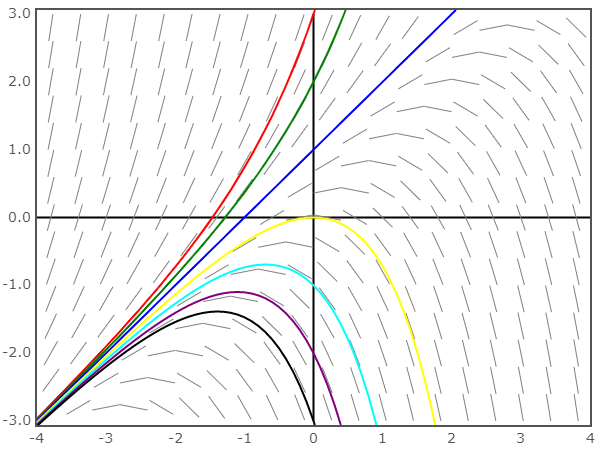
\includegraphics[width=0.8\textwidth]{images/y-t-slopefield.png}
    \end{center}
    \item What do your sketches suggest is the solution whose initial value is $y(0) = 1$? How does this connect to your work on problem \#2?
    
    \begin{red}
    It looks like this solution is linear, and indeed, the solution in \#2(b) was the linear function $y(t) = t+1$.
    \end{red}
    \item Draw a graph of the function $y(t) = t+1-2e^t$ from problem \#1. What's $y(0)$ for this function? How does this graph compare to the sketches you've made?
    
    \begin{red}
    $y(0) = 0+1-2e^0 = -1$, and indeed, the graph of this function matches the sketch I made of the solution whose initial value is $y(0) = -1$. (That's an annoying very light blue in the picture above.)
    \end{red}
    \item (Bonus question) Look at the points where each of these solutions has a local maximum. Notice anything interesting?

    \begin{minipage}{0.6\textwidth}    
    \begin{red}
    If the solution has a local maximum, then $\dfrac{dy}{dt}$ should be 0. So, since $\dfrac{dy}{dt} = y-t$, we can insist that $0 = y-t$ -- in other words, $y=t$. And indeed, if you draw the line $y=t$, which I've done in an annoying magenta color below, it goes smack dab through all of the local maxima of the solutions, including a bunch more that I added for illustration. (Neat! This is called the ``nullcline''.)
    \end{red}
    \end{minipage}
    \hfill
    \begin{minipage}{0.3\textwidth}
        \begin{center}
        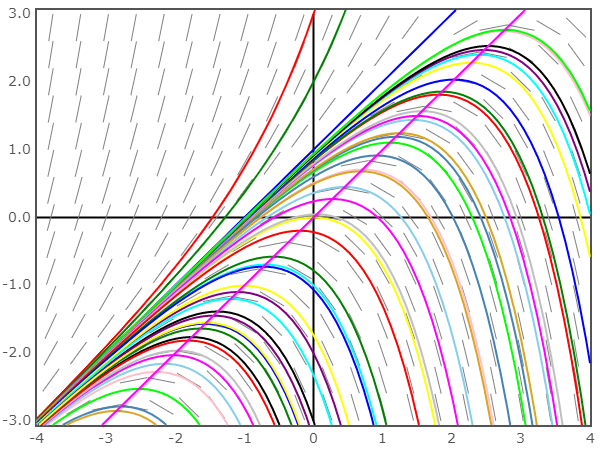
\includegraphics[width=\textwidth]{images/y-t-slopefield-maxes.png}
    \end{center}
    \end{minipage}
\end{enumerate}

\pagebreak

\item This differential equation isn't separable. Explain why not.

\begin{red}
Since the $y$ and the $t$ on the RHS are added / subtracted, I can't multiply or divide in order to get something of the form $g(y) \frac{dy}{dt} = h(t)$, where the LHS is a product of a function of $y$ only and $\frac{dy}{dt}$ and the RHS is a function of $t$ only.
\end{red}

Therefore, we don't have the tools to find a function that's a solution for this equation. Darn!

\begin{red}
As noted later, if you want to learn how to solve this equation, you can google the ``integrating factor method,'' or take a differential equations class.
\end{red}

\item (Modified from the work to produce \href{https://activecalculus.org/single/sec-7-3-euler.html#OcJ}{AC 7.3 Table 7.3.7}) Now we're going to approximate solutions numerically.
\begin{enumerate}
    \item Starting with the initial condition $y(0) = -1$, use Euler's method with $\Delta t = 0.2$ to approximate the solution at $t=0.2, 0.4, 0.6, 0.8, 1$. Record your work in this table:
    \[
    \begin{array}{|l|l|l|l|} 
    \hline
    \textrm{current } t & \textrm{current } y & \textrm{slope } \frac{dy}{dt} & \Delta y        \\\hline
    0                   & -1                  & \red{-1}                      & \red{-0.2}      \\\hline
    0.2                 & \red{-1.2}          & \red{-1.4}                    & \red{-0.28}     \\\hline
    0.4                 & \red{-1.48}         & \red{-1.88}                   & \red{-0.376}    \\\hline
    0.6                 & \red{-1.856}        & \red{-2.456}                  & \red{-0.4912}   \\\hline
    0.8                 & \red{-2.3472}       & \red{-3.1472}                 & \red{-0.62944}  \\\hline
    1.0                 & \red{-2.97664}      & \red{-3.97664}                & \red{-0.795328} \\\hline
    \end{array}
    \]
    
    \item Sketch each of these points on a graph. (Desmos might be fun.)

    \begin{red}
        See next page.
    \end{red}
    \item In \#3, you decided what the exact solution is to the initial value problem $\dfrac{dy}{dt} = y-t$, $y(0) = -1$. Use this exact solution to compute the actual -values at each of these points, and compute the error in your approximation at each of these points.
    
    \begin{red}
    We can compute actual $y$-values by plugging the current $t$-value into the function $y(t) = t+1-2e^t$.
    
    Here I'm reporting $y$-values and error values to five decimal places.
    \[
\begin{array}{|l|l|l|l|}
\hline
\textrm{current } t & \textrm{approx } y & \textrm{actual } y & \textrm{Error} \\ \hline
0                   & -1                 & -1                 & 0              \\ \hline
0.2                 & -1.2               & -1.24281           & 0.04281        \\ \hline
0.4                 & -1.48              & -1.58365           & 0.10365        \\ \hline
0.6                 & -1.856             & -2.04424           & 0.18824        \\ \hline
0.8                 & -2.3472            & -2.65108           & 0.30388        \\ \hline
1                   & -2.97664           & -3.43656           & 0.45992        \\ \hline
\end{array}
    \]
    \end{red}
    \item Sketch the exact solution on the same graph you drew your points on.
    
    \begin{red}
    See next page. I've also included the corresponding actual-values points on the actual solution function, as well as little bars indicating the error on each point. You can see that the numerical approximation is actually pretty good! and also that the goodness of the approximation really falls off as we step further out from the starting point.
    \end{red}
    
    \begin{center}
        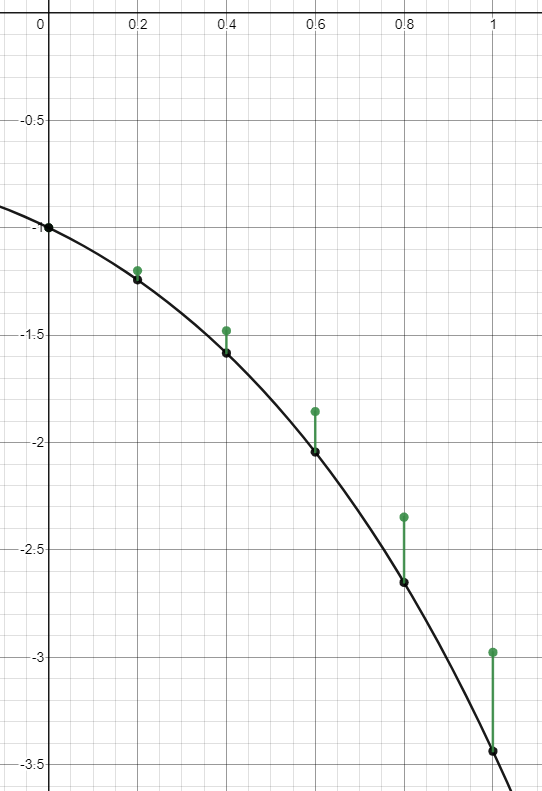
\includegraphics[width=0.8\textwidth]{images/euler-vs-actual.png}
    \end{center}
\end{enumerate}


\end{enumerate}
\pagebreak

\begin{blue}
FYI and in case you are curious but by no means do you need to know this for the purposes of MATH 202: here's a sketch of a solution using the ``integrating factor method.'' First I'll rewrite the equation in a ``standard form'' by getting all the $y$ stuff to the LHS:
\[\frac{dy}{dt} + (-1) y = -t\]
Now I will multiply both sides by something called the ``integrating factor,'' which in this case is $\exp(\int(-1)\, dt) = e^{-t}$:
\[e^{-t} \frac{dy}{dt} + (-e^{-t}) y = -t e^{-t}\]
The LHS is now in the shape of something that came out of the product rule (!!), because $-e^{-t}$ is the derivative of $e^{-t}$.
\[\frac{d}{dt} \left[ e^{-t} \cdot y \right] = -t e^{-t}\]
Integrate both sides with respect to $t$. Use integration by parts on the RHS. Then, solve for $y$ by dividing both sides by the integrating factor $e^{-t}$.
\[e^{-t}\cdot y = \int -te^{-t}\ dt = t e^{-t} + e^{-t} + C\]
\[y = t + 1 + \frac{C}{e^{-t}} = t + 1 + Ce^t\]
Then you can use an initial value to solve for the value of $C$. Check that $y(0) = -1$ produces $C = -2$.
\end{blue}

\end{document}